% Options for packages loaded elsewhere
\PassOptionsToPackage{unicode}{hyperref}
\PassOptionsToPackage{hyphens}{url}
%
\documentclass[
]{article}
\usepackage{amsmath,amssymb}
\usepackage{iftex}
\ifPDFTeX
  \usepackage[T1]{fontenc}
  \usepackage[utf8]{inputenc}
  \usepackage{textcomp} % provide euro and other symbols
\else % if luatex or xetex
  \usepackage{unicode-math} % this also loads fontspec
  \defaultfontfeatures{Scale=MatchLowercase}
  \defaultfontfeatures[\rmfamily]{Ligatures=TeX,Scale=1}
\fi
\usepackage{lmodern}
\ifPDFTeX\else
  % xetex/luatex font selection
\fi
% Use upquote if available, for straight quotes in verbatim environments
\IfFileExists{upquote.sty}{\usepackage{upquote}}{}
\IfFileExists{microtype.sty}{% use microtype if available
  \usepackage[]{microtype}
  \UseMicrotypeSet[protrusion]{basicmath} % disable protrusion for tt fonts
}{}
\makeatletter
\@ifundefined{KOMAClassName}{% if non-KOMA class
  \IfFileExists{parskip.sty}{%
    \usepackage{parskip}
  }{% else
    \setlength{\parindent}{0pt}
    \setlength{\parskip}{6pt plus 2pt minus 1pt}}
}{% if KOMA class
  \KOMAoptions{parskip=half}}
\makeatother
\usepackage{xcolor}
\usepackage[margin=1in]{geometry}
\usepackage{graphicx}
\makeatletter
\def\maxwidth{\ifdim\Gin@nat@width>\linewidth\linewidth\else\Gin@nat@width\fi}
\def\maxheight{\ifdim\Gin@nat@height>\textheight\textheight\else\Gin@nat@height\fi}
\makeatother
% Scale images if necessary, so that they will not overflow the page
% margins by default, and it is still possible to overwrite the defaults
% using explicit options in \includegraphics[width, height, ...]{}
\setkeys{Gin}{width=\maxwidth,height=\maxheight,keepaspectratio}
% Set default figure placement to htbp
\makeatletter
\def\fps@figure{htbp}
\makeatother
\setlength{\emergencystretch}{3em} % prevent overfull lines
\providecommand{\tightlist}{%
  \setlength{\itemsep}{0pt}\setlength{\parskip}{0pt}}
\setcounter{secnumdepth}{-\maxdimen} % remove section numbering
\ifLuaTeX
  \usepackage{selnolig}  % disable illegal ligatures
\fi
\usepackage{bookmark}
\IfFileExists{xurl.sty}{\usepackage{xurl}}{} % add URL line breaks if available
\urlstyle{same}
\hypersetup{
  pdftitle={Indirect Cost Forecasting},
  pdfauthor={Md Ismail Hossain},
  hidelinks,
  pdfcreator={LaTeX via pandoc}}

\title{Indirect Cost Forecasting}
\author{Md Ismail Hossain}
\date{2025-01-30}

\begin{document}
\maketitle

\subsection{R Markdown}\label{r-markdown}

\begin{verbatim}
## Registered S3 method overwritten by 'quantmod':
##   method            from
##   as.zoo.data.frame zoo
\end{verbatim}

\begin{verbatim}
## Warning: Using `size` aesthetic for lines was deprecated in ggplot2 3.4.0.
## i Please use `linewidth` instead.
## This warning is displayed once every 8 hours.
## Call `lifecycle::last_lifecycle_warnings()` to see where this warning was
## generated.
\end{verbatim}

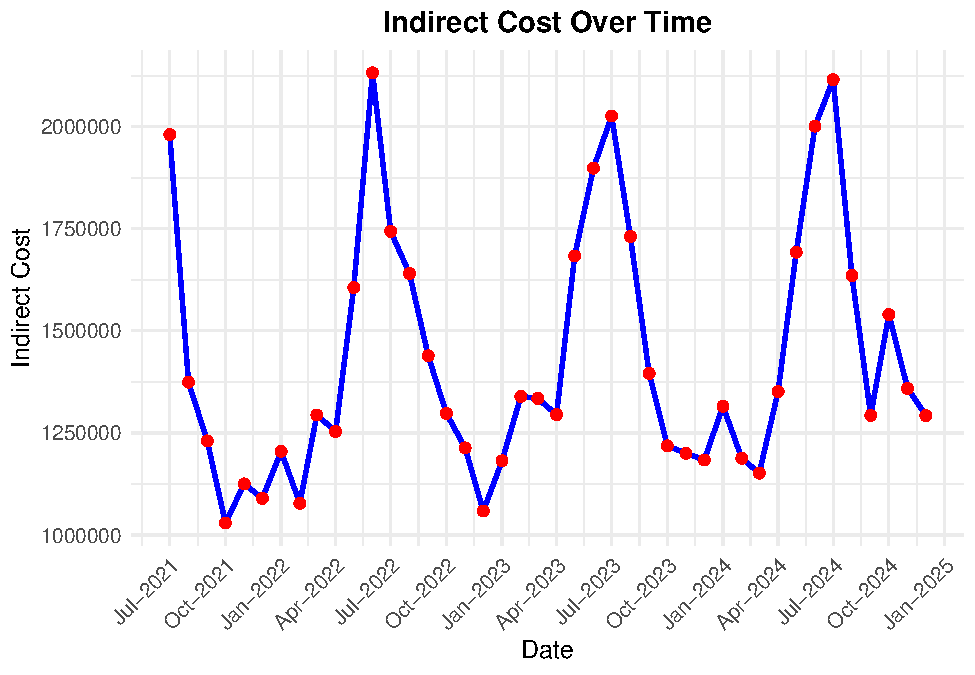
\includegraphics{Indirect-Cost-Forecasting-Report_files/figure-latex/unnamed-chunk-1-1.pdf}

\begin{verbatim}
## Series: ts_data 
## ARIMA(0,0,0)(1,1,0)[12] with drift 
## 
## Coefficients:
##          sar1     drift
##       -0.5272  4342.358
## s.e.   0.1834  1506.108
## 
## sigma^2 = 1.772e+10:  log likelihood = -397.46
## AIC=800.91   AICc=801.84   BIC=805.12
## 
## Training set error measures:
##                    ME     RMSE      MAE         MPE     MAPE      MASE
## Training set 1297.762 108693.3 73537.75 -0.04184224 5.003099 0.5620852
##                     ACF1
## Training set -0.04643894
\end{verbatim}

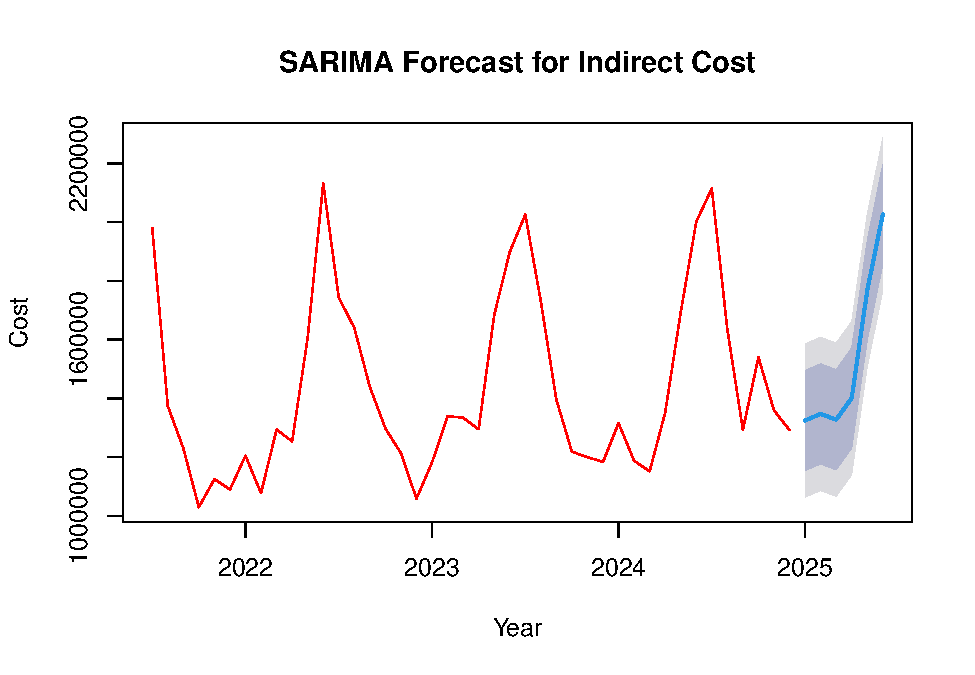
\includegraphics{Indirect-Cost-Forecasting-Report_files/figure-latex/unnamed-chunk-2-1.pdf}

\begin{verbatim}
##          Point Forecast   Lo 80   Hi 80   Lo 95   Hi 95
## Jan 2025        1324539 1153937 1495141 1063625 1585452
## Feb 2025        1347334 1176732 1517936 1086421 1608248
## Mar 2025        1327454 1156852 1498056 1066540 1588367
## Apr 2025        1401024 1230421 1571626 1140110 1661937
## May 2025        1767380 1596778 1937982 1506467 2028294
## Jun 2025        2026608 1856006 2197210 1765694 2287521
\end{verbatim}

\end{document}
